% TrackPilot 论文中文对照译本（对应 main.tex，2026-11-16 版）。
% 仅供作者阅读和改写时对照；投稿以英文版 main.tex 为准。数字与英文版逐一对应，来源见 main.tex 中各表旁的注释。
% 编译：cd paper && tectonic main_zh.tex（需要 XeTeX 和系统中文字体；Overleaf 上请选 XeLaTeX，并按需替换下面的字体名）。
\documentclass[webpdf,contemporary,large]{oup-authoring-template}

\usepackage{booktabs}
\usepackage{tikz}
\usetikzlibrary{arrows.meta,positioning}
\usepackage{xeCJK}
\setCJKmainfont[AutoFakeBold=2.5,AutoFakeSlant=0.15]{STSong}
\setCJKsansfont[AutoFakeBold=2.5]{Hiragino Sans GB}
\setCJKmonofont{Hiragino Sans GB}
\xeCJKsetup{CJKspace=false}
\renewcommand\figurename{图}
\renewcommand\tablename{表}
\renewcommand\refname{参考文献}
\newcommand{\todo}[1]{\textcolor{red}{[待补：#1]}}
\newcommand{\tp}{TrackPilot}
\linespread{1.08}

\journaltitle{Bioinformatics}
\DOI{DOI HERE}
\copyrightyear{2026}
\pubyear{2026}
\access{中文对照译本，仅供参考，以英文稿为准}
\appnotes{Original Paper}

\begin{document}

\title[TrackPilot]{TrackPilot：用少量实测变异，为一种细胞类型选择可信的基因组基础模型轨道}

\author[1,$\ast$]{\todo{第一作者}}
\author[1]{\todo{合作者}}
\authormark{\todo{作者} 等}
\address[1]{\orgdiv{\todo{院系}}, \orgname{\todo{单位}}, \orgaddress{\country{\todo{国家}}}}
\corresp[$\ast$]{通讯作者。\todo{邮箱}}

\received{Date}{0}{Year}
\revised{Date}{0}{Year}
\accepted{Date}{0}{Year}

\abstract{
\textbf{动机：}AlphaGenome 等序列—功能模型会针对一个变异，在约一千条细胞类型特异的轨道上给出效应预测。研究某一种细胞的实验室必须决定采用其中哪些预测。按细胞类型名称匹配轨道并不可靠，而且很多细胞类型根本没有被测绘。实验室在大规模研究之前常会先测少量变异，但目前既没有系统的方法来决定测哪些变异，也没有方法把少数几个测量值转化为对上千条相互关联的轨道的选择。\\
\textbf{结果：}我们提出 \tp{}。它把每条轨道看作一个假设：实验测量值是该轨道预测值的某个未知线性函数；它以闭式积分掉这一校准，并以元数据与该细胞类型匹配的轨道为起点。它提出一组试点变异，即各条可信轨道在其上意见分歧的变异，并为每个未测变异给出按后验加权的预测。我们在三个诱变报告基因实验上做了预注册检验。在 125 个位点上，8 个试点测量值不劣于匹配轨道（Spearman 相关均值 $+0.010$）；隐藏这些轨道后，比全轨道平均高 0.047（$P = 3\times10^{-12}$）；而 8 个随机测量值让同样的推断比不测还差。这一提升最早出现在早期版本于另一数据集上的预注册检验中。Siraj 的结果在第二个模型 Enformer 上、以及在未用这些位点训练的检查点上同样成立；Enformer 也重现了早期的提升。在没有自身轨道的细胞类型中，提升并不一致：试点变异组仍优于随机变异组，但在小鼠细胞系中 8 个测量值没有超过全轨道平均；在诱导神经元中，轨道几乎预测不了实验结果。对同一组测量值做置换检查后，可以退回不依赖标签的默认预测，挽回部分损失。\\
\textbf{可用性与实现：}\tp{} 是一个 Python 包和命令行工具（MIT 许可），见\newline
\url{https://github.com/ydvislab/AuraGenome-V} \todo{正式仓库名、PyPI 名称、投稿版本的 Zenodo DOI}。预注册文件和全部派生结果在同一仓库中。\\
\textbf{联系方式：}\todo{邮箱}\\
\textbf{补充信息：}补充材料见 \textit{Bioinformatics} 网站。}

\keywords{变异效应预测，基因组基础模型，主动模型选择，贝叶斯实验设计，大规模平行报告基因实验}

\maketitle

%===============================================================================
\section{引言}

深度序列—功能模型仅凭 DNA 序列就能预测非编码变异的调控后果
\citep{zhou2015deepsea,avsec2021enformer,linder2025borzoi}。其中最新的 AlphaGenome 为数百种人类细胞类型和组织预测数千条基因组轨道，并能在所有轨道上为任意单核苷酸变异打分 \citep{avsec2026alphagenome}。在 CAGI5 调控挑战等饱和诱变基准上 \citep{kircher2019saturation,shigaki2019cagi5}，它属于目前最好的预测器之一。然而，它对每个变异给出的不是一个预测，而是约一千个，每条轨道一个。

因此，研究某种细胞中变异的实验室必须选择用哪些轨道。通常的做法是选生物样本名称与细胞系一致的轨道。我们发现这并不可靠。在 AlphaGenome 的 1,018 条 CAGE、DNase 和 ATAC 轨道中，按与实测效应的一致程度排序，名称匹配的轨道在我们的开发元件上排在第 1 到第 27 位不等；而且这一选择会改变生物学结论：在 K562 细胞的 \textit{PKLR} 启动子上，把 K562 轨道换成 HepG2 轨道后，方向判断正确的显著变异比例从 0.96 降到 0.69--0.85。实验室使用的许多细胞类型，包括病人来源的细胞系，并没有被测绘，这时连可以匹配的名称都没有。把模型适配到新的细胞类型是可行的，但需要该细胞类型的全基因组图谱 \citep{hingerl2025scooby}。

实验室通常能做的是测少量变异，例如在大规模研究之前先做一个包含 8--16 个构建体的试点报告基因实验。于是，选择轨道就变成一个少标签模型选择问题：决定测哪些变异，使测量结果能够识别出最能预测其余变异的轨道或轨道组合 \citep{cohn1996active}。主动模型选择方法针对分类器解决了这一问题 \citep{karimi2021modelpicker,okanovic2025modelselector,kay2025coda}。基础模型轨道有两个特点，使这些方法的假设不再成立。第一，轨道是任意尺度上的回归输出，每条都要用一个未知的斜率和偏移校准到实验上，而少数几个标签无法把它们定准。第二，轨道是同一网络的上千个高度相关的输出头，少量标签往往无法确定哪一条最好 \citep{kuboyama2026labels}，对可信轨道做平均才能体现这种不确定性 \citep{hoeting1999bma}。这个问题并非 AlphaGenome 独有：任何有许多输出头的模型，加上一个只有少量标签的用户，都会遇到它。

本文提出 \tp{}，一个把少量实测变异转化为“用哪些轨道”这一决定的工具。\tp{}（i）把每条轨道看作带仿射校准的假设，并以闭式积分掉校准；（ii）从元数据匹配的轨道出发，只有当测量结果与它们矛盾时才偏离；（iii）用经典的模型判别准则选择要测的变异 \citep{box1967discrimination}；（iv）报告按后验加权的预测，而不是某一条被选中的轨道。我们在三个诱变报告基因数据集上做了预注册检验，依次回答三个问题：有匹配轨道时它是否比匹配轨道差；匹配轨道缺失时它能否找到替代；它在哪里不再有用。我们还把它与更简单的选点方式、少标签回归和主动模型选择做了比较，并检查了结论对模型训练暴露的依赖。

%===============================================================================
\section{方法}

\begin{figure*}[t]
\centering
\begin{minipage}[b]{0.335\textwidth}
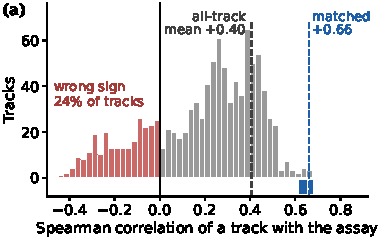
\includegraphics[width=\linewidth]{figures/fig1_problem.pdf}
\end{minipage}\hfill
\begin{minipage}[b]{0.645\textwidth}
\centering
\begin{tikzpicture}[node distance=0.45cm and 0.32cm, every node/.style={font=\scriptsize},
  box/.style={draw, rounded corners=2pt, align=center, inner sep=3pt, text width=2.3cm, minimum height=1.05cm},
  arr/.style={-{Stealth[length=1.6mm]}, thick}]
\node[box] (tracks) {模型预测\\ 变异 $\times$ 轨道\\（此处为 1,018 条 AlphaGenome 轨道）};
\node[box, right=of tracks] (prior) {轨道先验\\ 以元数据匹配的轨道为默认 + 轨道族};
\node[box, right=of prior] (post) {轨道后验\\ 校准参数 $a, b$\\ 被积分掉};
\node[box, right=of post] (pick) {\texttt{trackpilot suggest}\\ 试点变异组：各轨道意见分歧的变异};
\node[box, below=0.4cm of post, text width=4.6cm, minimum height=0.7cm] (out) {\texttt{trackpilot predict}\\
为每个未测变异给出按后验加权的预测};
\draw[arr] (tracks) -- (prior);
\draw[arr] (prior) -- (post);
\draw[arr] (post) -- (pick);
\draw[arr] (pick.north) to[out=135, in=45] node[above, align=center] {在实验中测量 $y_j$} (post.north);
\draw[arr] (post.south) -- (out.north);
\node[anchor=north west, font=\footnotesize\bfseries] at ([yshift=0.75cm]tracks.north west) {(b)};
\end{tikzpicture}
\end{minipage}
\caption{问题与 \tp{}。(a) 在 \textit{IRF4} 增强子（SK-MEL-28；图~\ref{fig:example}）的全部 1,353 个替换上，1,018 条 AlphaGenome 轨道各自与实测效应的 Spearman 相关（用全部标签计算）；24\% 的轨道预测的方向相反（红色）。刻度线：7 条匹配轨道；虚线：匹配轨道平均和全部轨道平均。(b) 每条轨道是一个假设：实测效应是该轨道预测的仿射函数。\tp{} 从偏向匹配轨道的先验出发，提出约 8 个各轨道意见分歧的变异，用它们的实测效应更新后验，再预测其余所有变异。}
\label{fig:overview}
\end{figure*}

\subsection{问题}

在细胞类型 $c$ 中研究一个调控元件。基础模型对每个候选变异 $j$ 在 $T$ 条轨道上各给出一个预测效应 $x_{t,j}$（此处 $T = 1{,}018$）。实验室可以测量 $k$ 个变异的效应 $y_j$；这些变异从一个可构建的变异池中选出，同时测量未突变的参照序列作为对照，使每个效应都是相对参照的。我们要为其余每个变异给出预测 $\hat y_j$，并找出能使这些预测尽可能准确的变异组 $S$（$|S| = k$）。准确度用变异池以外变异上 $\hat y$ 与 $y$ 的 Spearman 相关来衡量。

\subsection{轨道即带校准的假设}

每条轨道的预测在元件内缩放但不中心化，$z_{t,j} = x_{t,j}/\mathrm{sd}_j(x_{t,\cdot})$，使符号保留替代等位基因的方向。假设 $t$ 认为
\begin{equation}
\begin{aligned}
y_j &= a + b\,z_{t,j} + \varepsilon_j,\\
a &\sim N(0,\alpha s^2),\quad b \sim N(0,\beta s^2),\quad \varepsilon_j \sim N(0,(1-\beta)s^2),
\end{aligned}
\end{equation}
其中 $s^2$ 为 $y_S^2$ 的均值，是标签尺度的代入估计。给定 $s^2$，积分掉 $a$ 和 $b$ 后得到所测变异组的边际似然
\begin{equation}
y_S \mid t \sim N\!\left(0,\ s^2\left[(1-\beta)I + \alpha \mathbf{1}\mathbf{1}^\top + \beta z_{t,S} z_{t,S}^\top\right]\right),
\end{equation}
以及后验 $p(t \mid y_S) \propto p(t)\,p(y_S \mid t)$。预测均值 $m_{t,j} = E[y_j \mid t, y_S]$ 由高斯条件分布得到，\tp{} 报告贝叶斯模型平均 $\hat y_j = \sum_t p(t\mid y_S)\,m_{t,j}$ \citep{hoeting1999bma}。$\alpha = 0.1$ 和 $\beta = 0.5$ 在任何评估之前就已固定。

\subsection{元数据先验}

如果模型测绘过该细胞类型，元数据匹配轨道的平均就是一个很强的默认预测。\tp{} 把它作为一个额外的假设加入，占先验概率 $\pi = 0.95$，其斜率先验以一个正值为中心，$b \sim N(\sqrt{\beta}\,s,\ (\beta/4)\,s^2)$，因此斜率为负的先验概率约为 2\%。其余概率由各单条轨道分享。预测相关系数 $r \ge 0.9$ 的轨道归为一族（平均连接聚类，不使用标签），先验先在族之间平分，再在族内平分，因此一族近似重复的轨道合起来只占一条轨道的先验。没有匹配轨道时就没有默认假设，全部先验分给单条轨道。$\pi$ 在 Kircher 开发元件上选定，并在 Siraj 检验前冻结；与预注册检验不同，这一选择的规则并没有在开发运行前提交。

\subsection{选择试点变异组}

变异组从变异池中逐个构建。给定当前后验，下一个变异使各假设预测均值的后验加权方差 $\mathrm{Var}_{t \sim p(t\mid y_S)}[m_{t,j}]$ 除以期望残差方差后最大。这就是用于模型判别的 Box--Hill 准则 \citep{box1967discrimination,rainforth2024modern}。在没有任何标签时，由于斜率先验对称，所有预测均值都为零，所以第一步使用每条轨道的标准化预测。由于选择结果对测量值的依赖很弱（第~\ref{sec:panel}~节），\tp{} 也可以在测量之前一次性给出整组变异：把每个已选变异的标签替换为当前的后验平均预测即可。

\subsection{测量数量}

变异组大小 $k$ 由用户设定（默认为 8）。我们在检验前把 $k=8$ 定为一个实际预算，即常见试点规模（8--16 个构建体）的下限，而不是推导出的最小值，并报告 $k$ 从 2 到 16 的结果。标签很少时每条轨道的校准都定不准，后验可能追随噪声（第~\ref{sec:panel}~节）。

\subsection{适用性检查}

只有当某条轨道或某种轨道组合能跟上实验结果时，\tp{} 才可能有用。测完变异组后，\tp{} 把混合模型的对数证据 $\log\sum_t p(t)\,p(y_S\mid t)$ 与同一组标签做 200 次随机置换后的值相比。如果真实标签并不比打乱的标签解释得更好（置换 $P > 0.5$，这一阈值在开发单位上选定），\tp{} 就改为返回不依赖标签的默认预测。这是一条经验性的回退规则，而不是对“没有信号”的检验；在像我们的评估那样根据标签逐个选择变异组时，它的零分布只是近似的。

\subsection{实现}

\tp{} 是一个带命令行界面的 Python 包，可用 \texttt{pip} 从代码仓库安装。它的输入是一张预测效应表（变异 $\times$ 轨道）和轨道元数据，因此不绑定某一个模型；一个可选模块可以用用户自己的 API 密钥调用 AlphaGenome 为某个区域打分（尚未在软件包中用真实密钥运行过）。\texttt{trackpilot suggest} 从变异池中返回 $k$ 个试点变异，大小用 \texttt{-k} 设定，\texttt{--measured} 可以在已测标签的基础上再追加一轮。\texttt{trackpilot predict} 接受任意数量的实测效应，返回轨道后验、所有变异的预测、经过适用性检查后的预测以及一份报告。在笔记本电脑上，一个含 1,353 个变异、1,018 条轨道的元件不到 5 秒即可完成。一个脚本用软件包重算了第一次重复中全部 4,734 个冻结版 \tp{} 结果（Kircher 和 Siraj），结果完全一致。

\subsection{数据与预测}

\textbf{Kircher 等} \citep{kircher2019saturation} 用饱和诱变 MPRA 测量了 20 个疾病相关调控元件中所有可能的替换。我们使用其中在人类细胞中进行的 22 个实验（27,789 个变异）。来自 5 个区域的 5 个实验构成开发集；来自 11 个区域的另外 17 个实验构成检验集。在小鼠细胞系（Neuro-2a、MIN6、NIH/3T3；5 个区域）中进行的 6 个实验只在另一项单独的预注册检验中分析。
\textbf{Siraj 等} \citep{siraj2026functional,siraj2025data} 在 K562 和 HepG2 细胞中测量了精细定位的性状变异周围 200 bp 寡核苷酸中的所有替换。我们使用了已发表的 128 个位点中的 125 个（一个因参照序列中存在缺失而排除，两个因在 GRCh38 中没有唯一匹配而排除），共 74,975 个替换，每个替换都在两种细胞中各测一次。效应定义为替换后寡核苷酸的 log$_2$ 倍数变化减去同一实验中未突变参照寡核苷酸的 log$_2$ 倍数变化；实验室在测试点变异组时也会构建这个参照。
\textbf{Kosicki 等} \citep{kosicki2025mpra} 在 iPSC 诱导的兴奋性神经元中，对 270 bp 片段每隔四个碱基做了合成颠换（ENCSR548AQS）：我们使用其中至少含 30 个替换的 328 个片段（22,397 个测量值），分布在 159 个区域，效应相对参照片段计算。有 4 条 AlphaGenome 轨道和 2 条 Enformer 轨道与神经元匹配。
\textbf{预测。}我们用 AlphaGenome（1 Mb 上下文，默认的蒸馏检查点）对每个变异做计算机诱变，覆盖人类生物样本的全部 CAGE、DNase 和 ATAC 轨道 \citep{avsec2026alphagenome}，这些轨道来自 ENCODE 和 FANTOM5 \citep{encode2020expanded,fantom2014atlas}。神经元区域用同样方式打分。为第~\ref{sec:general}~节，我们还用 Enformer \citep{avsec2021enformer} 在其 1,322 条人类 CAGE、DNase 和 ATAC 轨道上（196 kb 上下文，一次前向计算）为 11 个 Kircher 检验区域、小鼠细胞区域、随机抽取的 40 个 Siraj 位点和神经元区域打分。两种模型使用相同的分数：以变异为中心的 501 bp 窗口内信号总和的 log$_2$ 变化。

\subsection{评估设计}
\label{sec:eval}

\textbf{场景。}我们通过隐藏轨道来模拟三种情形：\emph{已测绘}，保留全部轨道；\emph{仅有相近细胞}，隐藏元件自身的细胞系；\emph{未测绘}，隐藏自身细胞类型和相近细胞类型。相近细胞类型在看到任何结果之前就根据轨道元数据列出。这些场景模拟的是缺失的细胞类型；真正没有轨道的细胞类型另行分析（第~\ref{sec:unprofiled}~节）。
\textbf{流程。}在 200 次重复中，每次取元件一半的变异作为可测的变异池。所有方法都在池外相同的变异上按 Spearman 相关打分。分析单位是区域（Kircher；同一区域的多个实验取平均）或位点（Siraj；两种细胞取平均）。
\textbf{预注册。}下面的每项检验都在运行前连同冻结的代码一起提交；如果所用数据此前已分析过，我们会注明。有两项分析在首次运行后做了更正，参数和判据不变，判定结果也相同：Kircher 改用共同评估集，Siraj 改用相对参照的效应（主要对比的变化分别不超过 0.004 和 0.002；补充表~S1）。
Kircher（不含元数据先验的版本）：H1，试点变异组优于随机变异组；H2，比全轨道平均至少高 0.03，且 11 个区域中至少 7 个差值为正。Siraj（冻结的 \tp{}）：P1，已测绘场景下 $k=8$ 时不劣于匹配轨道平均（单侧 95\% bootstrap 下界高于 $-0.02$）；P2，差值低于 $-0.05$ 的位点不超过 15\%；P3，未测绘场景下 $k=8$ 时比全轨道平均至少高 0.03；P4，仅有相近细胞场景下 $k=16$ 时优于相近细胞平均。神经元（N1--N4）和小鼠细胞实验（M1--M3）使用这些假设在 $k=8$ 时的对应版本（补充表~S10、S14）；适用性检查使用 A1 和 A2（第~\ref{sec:boundary}~节）。之后补充的分析均标为事后分析。
\textbf{训练数据、检验集与同源性。}\tp{} 不训练任何模型；AlphaGenome 以冻结状态使用，唯一的标签是被预测元件的 $k$ 个实测变异。在单位点分析中，其他元件的测量值和评估变异都不进入推断。检验集在分析前确定，与开发区域不重叠。AlphaGenome 的训练轨道确实覆盖这些区域，因此我们为每个位点换用一个检查点重做检验：该检查点的留出折包含与该位点重叠的所有训练窗口（\texttt{alphagenome.data.fold\_intervals}）。这些折就是 Borzoi 的划分，它把基因组片段随机分到 8 个折中，同时让人和小鼠的直系同源区域留在同一折 \citep{linder2025borzoi}。人类基因组内部的同源序列没有被显式归组，因此留出折的结果只是减少、而不是消除了训练暴露。
\textbf{基线。}不用标签的：全轨道平均、匹配轨道平均和相近细胞平均。其他选点方式：随机、预测效应最大、未加权分歧最大。少标签回归：在全部轨道上做岭回归 \citep{hoerl1970ridge} 和 LASSO \citep{tibshirani1996lasso}；对匹配轨道平均做仿射重拟合（\texttt{matched\_cal}）；对校准后的匹配轨道平均的残差做岭回归（\texttt{meta\_ridge}）。主动模型选择：CODA 式和 MODEL SELECTOR 式选择 \citep{kay2025coda,okanovic2025modelselector}，使用我们的校准似然。用全部标签选出的最佳单条轨道作为参考一并报告。

%===============================================================================
\section{结果}

\subsection{有匹配轨道时，\tp{} 不劣于它们}

在已测绘的细胞类型中，匹配轨道是自然的默认选择，所以第一条要求是不比它们差。在 Siraj 上保留全部轨道时，8 个测量值不劣于匹配轨道平均（P1：$+0.010$，单侧下界 $+0.005$，界值为 $-0.02$），只有 3/125 个位点差了 0.05 以上（P2：上界 6.1\%，界值 15\%；表~\ref{tab:siraj}，图~\ref{fig:siraj}）。$k=16$ 时差值为 $+0.019$，有一个位点受损。

元数据先验正是为这一要求而加入的，因此 Kircher 数据无法检验它。采用均匀先验的第一个版本通过了第~\ref{sec:substitute}~节的 Kircher 检验，但在保留匹配轨道时，它在同样的区域上比匹配轨道平均低 0.029，11 个区域中 7 个受损（事后分析）：它在匹配轨道不准的地方有帮助（\textit{LDLR}：匹配轨道平均 0.24，\tp{} 0.51），在匹配轨道准的地方却吃亏（\textit{SORT1}：0.65 对 0.48）。我们随后加入先验，在开发元件上选定 $\pi$，并在 Siraj 检验前冻结；在 Kircher 检验区域上，它与匹配轨道平均持平（$+0.001$，描述性结果）。最直接的捷径，即用同样几个标签重新拟合匹配轨道平均，在 Siraj 上降低了准确度（随机变异组 $-0.082$，试点变异组 $-0.010$），因为拟合出的斜率定不准，还可能变号。对匹配轨道平均的残差做岭回归（\texttt{meta\_ridge}）与 \tp{} 接近（$-0.007$；表~\ref{tab:siraj}，S2）。

\begin{table*}[t]
\centering
% results/a1/siraj_ref/siraj_decision.txt, siraj_secondary.tsv
\caption{Siraj 预注册检验，冻结的 \tp{}，125 个位点（每个位点对两种细胞取平均）。$D$ 为 Spearman 相关的平均配对差值。S 行为次要分析。}
\label{tab:siraj}
\begin{tabular}{llcc}
\toprule
假设 & 比较 & $D$ & 判据与结果 \\
\midrule
P1 & 已测绘，$k=8$：\tp{} $-$ 匹配轨道平均 & $+0.010$ & 下界 $+0.005 > -0.02$，成立 \\
P2 & 已测绘，$k=8$：$D<-0.05$ 的位点 & 3/125 & 上界 $0.061 \le 0.15$，成立 \\
P3 & 未测绘，$k=8$：\tp{} $-$ 全轨道平均 & $+0.047$ & $\ge 0.03$，$P=3\!\times\!10^{-12}$，成立 \\
P4 & 仅有相近细胞，$k=16$：\tp{} $-$ 相近细胞平均 & $+0.040$ & $>0$，$P=3\!\times\!10^{-19}$，成立 \\
\midrule
S1 & 未测绘，$k=8$：试点 $-$ 随机变异组 & $+0.096$ & 122/125 $>0$ \\
S2 & 已测绘，$k=8$：\tp{} $-$ \texttt{meta\_ridge} & $+0.007$ & 97/125 $>0$ \\
S3 & 已测绘，$k=8$：\texttt{matched\_cal}（随机变异组）$-$ 匹配轨道 & $-0.082$ & 1/125 $>0$ \\
\bottomrule
\end{tabular}
\end{table*}

\begin{figure*}[t]
\centering
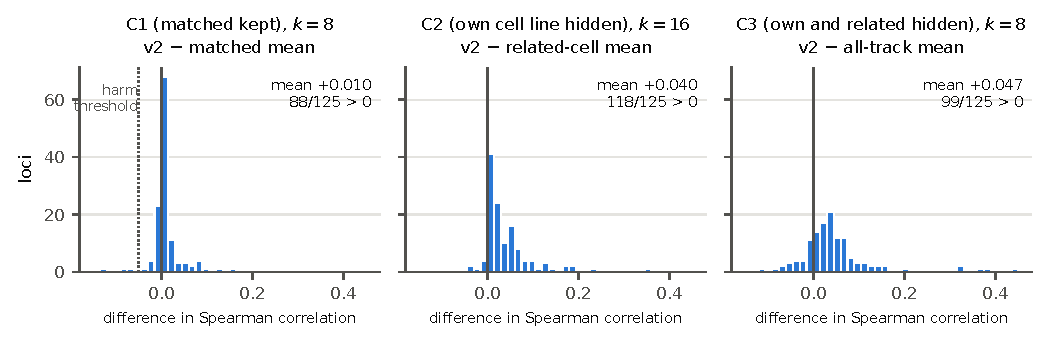
\includegraphics[width=\textwidth]{figures/fig_siraj.pdf}
\caption{125 个 Siraj 位点上各预注册比较的逐位点配对差值。虚线：预注册的受损阈值（$-0.05$）。}
\label{fig:siraj}
\end{figure*}

\subsection{匹配轨道缺失时，8 个测量值就能找到替代}
\label{sec:substitute}

隐藏元件自身及相近细胞类型的轨道后，不用标签的替代方案是全部轨道的平均。在 Siraj 上，8 个测量值比它高 0.047（0.391 到 0.438；$P = 3\times10^{-12}$；P3）。只有相近细胞轨道时，16 个测量值比它们的平均高 0.040（0.412 到 0.452；$P = 3\times10^{-19}$；P4）。元件、细胞系和实验设计都不同的 Kircher 检验得出一致结论：8 个试点测量值把平均 Spearman 相关从 0.296（全轨道平均）提高到 0.370，而 8 个随机测量值只有 0.286（表~\ref{tab:kircher}；补充图~S1）。两条预注册假设都成立：试点变异组比随机变异组高 0.084（11 个区域中 9 个为正，$P = 0.0024$），比全轨道平均高 0.074（8/11 个区域）。

提升集中在默认预测较差的地方（事后分析）：在全轨道平均离最佳轨道最远的四分之一 Siraj 位点上提升 0.133，在最近的四分之一上只有 0.004（补充表~S8）。图~\ref{fig:example} 展示了一次运行：SK-MEL-28 黑色素瘤细胞中的 \textit{IRF4} 增强子，黑色素细胞及相近轨道被隐藏。测了 8 个变异之后，后验偏向神经嵴细胞的 DNase 轨道（黑色素细胞正是由神经嵴发育而来），预测在留出变异上达到 $\rho = 0.59$，而全轨道平均为 0.39。

\begin{table*}[t]
\centering
% results/a1/common_eval_test_k8_by_element.tsv (region means), common_eval_test_decision.txt,
% common_eval_regression_baselines_k8.tsv
\caption{Kircher 检验集，未测绘场景（隐藏自身及相近细胞类型），$k=8$，11 个区域。数值为留出变异上的 Spearman 相关。预注册版本（均匀先验）；该场景下元数据先验不起作用。$^\dagger$事后分析（前 50 次重复）；LASSO 的范围涵盖处理全零拟合的三种规则。}
\label{tab:kircher}
\begin{tabular}{llccc}
\toprule
变异组 & 预测方式 & 平均 $\rho$ & \tp{} $-$ 本行 & 为正的区域数，单侧 $P$ \\
\midrule
试点（\tp{}） & 轨道后验 & 0.370 & --- & --- \\
随机 & 轨道后验 & 0.286 & $+0.084$ & 9/11，0.0024 \\
预测效应最大 & 轨道后验 & 0.338 & $+0.031$ & --，0.18 \\
无 & 全轨道平均 & 0.296 & $+0.074$ & 8/11，-- \\
随机 & LASSO$^\dagger$ & -- & $+0.110$ 至 $+0.182$ & 9--10/11，$\le$0.0024 \\
随机 & 岭回归$^\dagger$ & -- & $+0.116$ & 8/11，0.0068 \\
试点 & LASSO$^\dagger$ & -- & $+0.034$ 至 $+0.048$ & 8/11，$\le$0.016 \\
试点 & 岭回归$^\dagger$ & -- & $+0.023$ & 8/11，0.042 \\
全部标签 & 最佳单条轨道（参考） & 0.454 & --- & --- \\
\bottomrule
\end{tabular}
\end{table*}

\begin{figure*}[t]
\centering
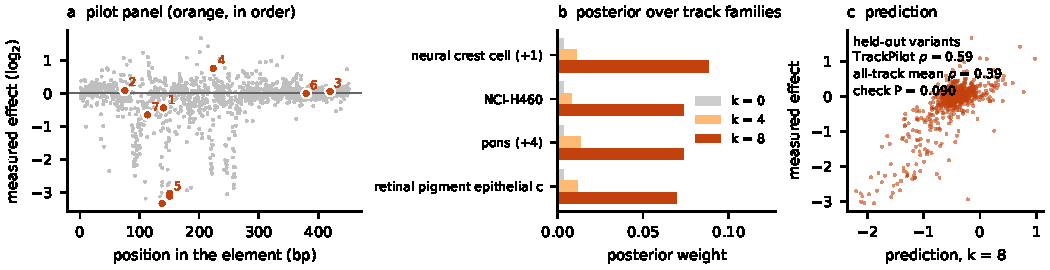
\includegraphics[width=\textwidth]{figures/fig_worked_example.pdf}
\caption{实例：SK-MEL-28 中的 \textit{IRF4} 增强子，黑色素细胞及相近轨道被隐藏，AlphaGenome，一次重复。(a) 实测效应；橙色为按顺序选出的试点变异。(b) 测了 0、4、8 个变异后，排名前四的轨道族的后验权重。(c) 留出变异的实测值对预测值。}
\label{fig:example}
\end{figure*}

\subsection{测哪些、测多少很重要；一轮选完与逐个选择一样好}
\label{sec:panel}

测随机变异比不测还差：在 Siraj 的未测绘场景下，同样的推断用随机变异组只达到 0.342，低于不用标签的全轨道平均（0.391），而试点变异组在 122/125 个位点上优于随机变异组（S1）。具体用哪个准则则没那么重要：按“哪条轨道正确”的期望信息增益来选，与试点变异组相当（差值 $\le 0.003$；事后分析；补充表~S4、S6）。保留匹配轨道时，选预测效应最大的变异同样好，但没有匹配轨道时更差（Siraj 未测绘：$-0.028$，97/125 个位点）。最有实际意义的是：在任何测量之前一轮选完的变异组，在两个数据集上都与逐个选择相差不超过 0.005，在我们事先声明的 0.02 等价界值之内。因此实验室可以一次订购整组构建体。准确度随 $k$ 上升（Siraj，隐藏匹配轨道，事后分析；补充表~S7）：2 个测量值低于不用标签的默认预测（0.347 对 0.391），4 个就超过了它（0.402），与 16 个随机测量值相当（0.404），8 个和 16 个分别达到 0.438 和 0.461。有匹配轨道时默认预测更强，需要 8 个测量值才能超过它（0.483 对 0.474；4 个时为 0.469）。

\subsection{与回归和主动模型选择的比较}

用同样 8 个标签，在全部轨道上做回归远不如 \tp{}（表~\ref{tab:kircher}）；即使在试点变异组本身上，\tp{} 的推断仍比 LASSO 和岭回归高 0.023--0.048。与使用我们校准似然的主动模型选择相比（CODA 的先验权重在开发元件上固定；事后分析；补充表~S5），\tp{} 在保留匹配轨道的 Siraj 上比 CODA 式选出的单条轨道高 0.075（111/125 个位点），没有匹配轨道时高 0.029--0.034，在 Kircher 上高 0.051--0.082。让基线报告后验平均而不是单条轨道，可以挽回 0.016--0.026；隐藏匹配轨道时，\tp{} 相对这一平均版基线仍有小幅优势（Siraj $+0.018$，95\% 区间 0.011--0.024），而同一基线换成均匀先验后与 \tp{} 持平（相差不超过 0.006）。这些比较支持对校准后的轨道做平均以及使用元数据先验；它们没有显示我们的选点准则比期望信息增益有多少优势。

\subsection{第二个基础模型}
\label{sec:general}

\tp{} 只使用预测矩阵和轨道元数据，因此我们在 Enformer 的预测上原样重新运行了冻结的方法。假设和阈值与 AlphaGenome 检验相同，并在打分前提交；为节省计算，Siraj 只用了随机抽取的 40 个位点。六条假设全部成立（补充表~S15）。有匹配轨道时，8 个测量值不劣于它们（$+0.022$，单侧下界 $+0.007$；1/40 个位点差了 0.05 以上）。没有匹配轨道时，8 个测量值在 Siraj 上比全轨道平均高 0.052（$P = 4\times10^{-4}$），在 Kircher 上高 0.109（8/11 个区域），比 8 个随机测量值高 0.097（10/11 个区域，$P = 0.001$）。两个模型都用这些区域以及 K562 和 HepG2 训练过，所以这里检验的是换模型，而不是换细胞类型。

\subsection{稳健性}

\textbf{训练暴露。}默认检查点是从在全部训练折上训练的教师模型蒸馏而来的，因此见过每个被检验位点上的轨道 \citep{avsec2026alphagenome}。我们为每个位点换用留出其所在基因组折的 AlphaGenome 检查点，重做了两项检验，判读规则在运行前提交。绝对准确度下降了 0.035--0.07，匹配轨道下降最多（Siraj：0.474 降到 0.402）。Siraj 的四条假设仍全部成立，且效应更大（P1 $+0.024$，P3 $+0.050$，P4 $+0.053$；补充表~S3）。在 11 个 Kircher 区域上，试点变异组相对随机变异组的优势增大（$+0.093$，10/11，$P = 0.0015$），相对全轨道平均的优势缩小（$+0.054$，$P = 0.062$），因此按事先提交的规则，Kircher 的结果依赖训练暴露。
\textbf{效应方向。}在 Siraj 上，方向准确率与排序结果一致；在 Kircher 上，\tp{} 判断对的方向比匹配轨道平均少（$-0.133$；去掉拟合的偏移后为 $-0.071$，因此 \tp{} 也报告这一版本；补充表~S2）。
\textbf{跨位点共享。}从同一细胞类型的另外 10 个位点汇集出的先验，在隐藏匹配轨道的 85 个位点上增加了 0.012，低于预注册的 0.02（补充表~S9）。

\subsection{没有自身轨道的细胞类型}
\label{sec:unprofiled}

隐藏已测绘细胞类型的轨道后，通常还会留下一条相近的轨道。下面三项检验针对的是本身就没有轨道的细胞类型。

Kircher 检验集中有 5 个区域是在没有自身轨道的人类细胞系中测的（HEL 92.1.7、SK-MEL-28 和三个胶质母细胞瘤细胞系），每个都在运行前指定了一个相近的生物样本作为代理。在这些区域上（事后分析），\tp{} 保持了代理的准确度（AlphaGenome $+0.002$，Enformer $+0.010$）；隐藏代理后，比全轨道平均高 0.12 和 0.16（3/5 和 4/5 个区域），比随机变异组高 0.10--0.11（5/5；补充表~S13）。

随后我们对 Kircher 中在小鼠细胞系（Neuro-2a、MIN6、NIH/3T3）里测的 5 个区域做了预注册检验。没有任何人类轨道测绘过这些细胞，代理是根据元数据指定的人类细胞。两个模型的结果都不支持假设（补充表~S14）。隐藏代理后，试点变异组优于随机变异组（AlphaGenome $+0.086$，Enformer $+0.102$），但没有优于全轨道平均（$-0.004$，$+0.022$；要求 0.03）。保留代理时，\tp{} 纠正了一个差的代理（\textit{ZFAND3}：$+0.17$，$+0.14$），但在 AlphaGenome 的 \textit{RET} 上损失 0.068，那里代理已接近最佳轨道。最佳单条轨道达到 0.30--0.34，说明信号是存在的，但 8 个测量值没能稳定地找到它；用 16 个测量值时（事后分析），相对全轨道平均的差值增大到 $+0.019$ 和 $+0.040$。

在模型几乎没有测绘的诱导神经元中，预注册检验（N1--N4，两个模型）因另一个原因失败：轨道几乎预测不了实验结果。匹配轨道的 Spearman 相关为 0.07，全轨道平均为 0.04--0.05；\tp{} 比匹配轨道平均低 0.02--0.03，比全轨道平均低 0.01--0.04，约 30\% 的区域差了 0.05 以上（补充表~S10）。

\subsection{测量结果与任何轨道都不符时的回退}
\label{sec:boundary}

用户在测量前看不到轨道的准确度，但可以把 8 个标签的拟合程度与打乱后的副本相比。因此我们预注册了适用性检查，并在逐个选择的变异组上评估：它的阈值在三个数据集的开发单位上选定（5 个 Kircher 实验、40 个 Siraj 位点、50 个神经元区域），并在运行留出单位之前提交。在 109 个留出的神经元区域上，它在 43--46\% 的运行中回退，比未经检查的 \tp{} 提高 0.010（65/109 个区域，$P = 0.002$；A1），与默认预测相差不超过 0.004。在 85 个留出的 Siraj 位点上，它只在 5--8\% 的运行中介入，并保住了提升：没有匹配轨道时比全轨道平均高 $+0.056$，有匹配轨道时比匹配轨道平均高 $+0.011$（A2；补充表~S11）。所有留出单位此前都分析过，只是没有参与阈值的选择；神经元的总体结果也正是促成这一检查的原因，所以 A1 是较弱的证据。使用 Enformer 预测时（次要分析），检查比未经检查的 \tp{} 高 0.019，但仍比默认预测低 0.015：此时置换 $P$ 值接近均匀分布，约一半的运行碰巧通过。更严格的阈值（0.2，一个可选项）在开发单位上同样好，把这一损失降到 $\le 0.007$，在 Siraj 上的代价 $\le 0.004$（事后分析；补充表~S12）。

%===============================================================================
\section{讨论}

\tp{} 为实验室在自己的细胞类型中使用基础模型提供了一套具体流程：从元数据匹配的轨道出发，测约 8 个经过挑选、能区分相互竞争的轨道的变异，只有当测量结果与默认预测矛盾时才让它们改变预测。支持这一流程的证据分三层。有匹配轨道时，在预注册的 Siraj 检验中，按排序相关它平均不劣于匹配轨道，两个模型都是如此；但在神经元中并非如此，那里轨道几乎预测不了实验结果。匹配轨道缺失、但其他细胞类型的轨道带有信号时，它在 Siraj 上把 Spearman 相关提高了 0.04--0.05，在 Kircher 上提高更多，两个模型都成立，在 Siraj 上换用留出检查点也成立。在没有自身轨道的细胞类型中，它挑出的变异仍优于随机，但 8 个测量值没能稳定地超过全轨道平均；在轨道几乎预测不了实验结果的地方，适用性检查在约一半的运行中退回默认预测。测量数量是用户手中的主要调节手段：只有 2 到 4 个标签时，预测可能低于默认预测；超过 8 个后准确度继续上升，在没有相近轨道的情况下上升最多，这时做第二轮是值得的。

三条经验看来具有普遍性：测哪些变异与如何建模同样重要；用少数几个标签重新拟合默认预测器是有害的，而以默认预测为中心的先验（在 Kircher 上看到这类损失后加入）在 Siraj 检验中避免了这些损失；在上千个相关的输出头中，后验平均优于最可能的单条轨道。

\textbf{局限性。}主要的提升是通过隐藏已测绘细胞类型的轨道测出来的。对于没有自身轨道的细胞类型，唯一的正面证据是事后分析，只覆盖 5 个区域；在小鼠细胞系中的预注册检验不支持假设。只有 8 个标签时，适用性检查的检验效能有限。评估是回顾性的，但在任何标签之前一轮选完的变异组同样准确（第~\ref{sec:panel}~节），因此实验室可以一次订购整组；回退规则只在逐个选择的变异组上评估过。平均不劣并不排除单个位点上的损失（3/125 个位点差了 0.05 以上，最大为 $-0.13$；单看一种细胞为 $-0.26$）。绝对相关只是中等水平（Siraj 上为 0.44--0.49）。只有当至少一条轨道或某种轨道组合大致与实验结果成比例时，\tp{} 才能有所帮助。

%===============================================================================
\section{结论}

只要决定从元数据默认出发、测量的变异是为区分轨道而挑选的、并且有某条接近该细胞类型的轨道带有实验信号，少量挑选得当的测量值就能指导我们在上千条基础模型轨道中依靠哪些；对于与所有已测绘细胞类型都相距甚远的细胞类型，则需要更多测量或新的图谱。\tp{} 把这件事变成两条命令；当测量结果与任何轨道的吻合都不比打乱的标签更好时，它会退回默认预测。

\section*{致谢}
\todo{致谢}
\todo{AI 使用声明（期刊 LLM 政策）；正文须由作者改写。}

\section*{作者贡献}
\todo{每位作者的 CRediT 角色}

\section*{资助}
\todo{资助}

\section*{利益冲突}
无。

\section*{数据可用性}
Kircher 等的数据存放于 GEO（GSE126550）\citep{kircher2019saturation}；我们使用的是作者在 \url{https://github.com/kircherlab/MPRA_SaturationMutagenesis} 发布的效应估计。Siraj 等的饱和诱变数据以 CC-BY-NC 许可发布于 Zenodo \citep{siraj2025data}，本文不再分发。神经元 MPRA 数据为 ENCODE 实验 ENCSR548AQS（文件 ENCFF958ZLG 和 ENCFF752NFF，CC BY 4.0）\citep{kosicki2025mpra}。预测可用仓库中的脚本重新生成。预注册文件、代码和所有派生表格见 \url{https://github.com/ydvislab/AuraGenome-V}。

\bibliographystyle{plainnat}
\bibliography{refs}

\end{document}
